\subsection{Фаза разметки текста}

\subsubsection{Скрытая марковская модель}
Скрытая марковская модель (CMM) - статистическая модель, широко применяемая в задачах распознавания речи, биоинформатики, сжатия данных, а также в области искуственного ителлекта. Процессы, протекающие в реальном мире проявляются в виде сигналов, воспринимаемых наблюдателем. Нередко источник сигналов непостижим наблюдателем в явном виде. Наблюдатель может судить о состоянии источника сигнала лишь по полученным сигналам, которые могут быть подвержены влиянию шумов, вследствие чего задача определения состояния источника сигналов становится нетривиальной. СММ является вероятностной моделью, широко применяемой в задачах определения внутреннего состояния процессу по его внешним проявлениям. СММ представляет собой обучаемый стохастический конечный автомат и может быть рассмотрены как специфическая форма динамической байесовской сети.

Впервые скрытые марковские модели начали применяться в области распознавания речи. Историю СММ можно разделить на две части.\cite{kouemou} С одной стороны это история Марковского процесса и Марковских цепей, а с другой - история алгоритмов, разрабатывавшихся для решений различных задач с помощью СММ. Андрей Андреевич Марков описал Марковские цепи в 1906 г., когда получил первые теоретические результаты исследования стохастических процессов. Марковский процесс может быть рассмотрен как процесс изменения некоторой случайной величины, который удовлетворяет Марковскому свойству. Марковское свойство заключается в том, что условное распределение вероятностей будущих состояний зависит от состояния, в котором процесс находится на данный момент, и не зависит от предыстории состояний. Другими словами, будущее не зависит от прошлого и зависит только от настоящего. В 1940-е годы с бурным развитием компьютерных наук многие ученые из разных областей начали искать применение как детерменированных, так и стохастических автоматов для решения своих задач. В 1977 году были обобщены накопившиеся знания и опыт использования EM-алгоритма\cite{dempster1977maximum}. 

EM-алгоритм является классическим алгоритмом, используемым в математической статистике для нахождения максимально правдоподобной оценки неизвестных параметров вероятностных моделей. EM-алгоритм представляет собой итеративный алгоритм.Каждая итерация алгоритма состоит из двух шагов. На E-шаге (expectation) вычисляется ожидаемое значение функции правдоподобия, при этом скрытые переменные рассматриваются как наблюдаемые. На M-шаге (maximization) вычисляется оценка максимального правдоподобия, таким образом увеличивается ожидаемое правдоподобие, вычисляемое на E-шаге. Затем это значение используется для E-шага на следующей итерации. Алгоритм выполняется до сходимости. Алгоритм Баума-Велша является частным случаем EM-алгоритма и применяется для нахождения неизвестных параметров скрытой марковской модели. Алгоритм Витерби был предложен Эндрю Витерби в 1967 году для декодирования сверточных кодов\cite{viterbi1967error}. Этот алгоритм относится к классу алгоритмов динамического программирования и позволяет найти наиболее правдоподобную последовательность скрытых состояний процесса, называемую путем Витерби.

\paragraph{Математическая модель}
Скрытая марковская модель представляет собой обучаемый стохастический конечный автомат. Выделяют два вида СММ: для дискретных наблюдений(событий) и непрерывных сигналов. В работе рассмотрена дискретная СММ ввиду дискретного характера данных, что будет обосновано далее. Скрытая марковская модель объединяет в себе два стохастических процесса.
\begin{enumerate}
\item
Первый процесс представляет собой переходы между состояними, скрытыми от наблюдателя.
\item
Второй процесс представляет собой пояление некоторый событий, которые известны наблюдателю. Распределения вероятностей появления этих событий зависят от скрытого состояния, в котором находится система.
\end{enumerate}


Формальо модель может быть описана следующими математическими объектами:
\begin{enumerate}
	\item
	Количество скрытых состояний модели \(N\). Несмотря на то, что информация о том, в каком состоянии модель находится в конкретный момент времени, не доступна для наблюдателя, множество всевозможных состояний наблюдателю извествно:
	множеством скрытых состояний
	\[ S = \{ S_1, S_2, ..., S_N \};\]
	\item
	Количество различных символов наблюдений \(M\). Символы наблюдений соответствуют регистрируемым событиям, попрождаемым наблюдаемым процессом. Множество различных символов наблюдений называется алфавитом наблюдений
	\[ V = \{ v_1, v_2, ..., v_M \};\]
	\item
	Матрицей вероятностей переходов между скрытыми состояниями
	\begin{align} 
		&A = \{ a_{ij} \}, \nonumber \\
		&a_{ij} = P[q_{t + 1} = S_j | q_t = S_i]; \nonumber
	\end{align}
	\item
	Распределение вероятностей появления символов в j-ом состоянии
	\begin{align}
		&B = \{ b_j(k) \}; \nonumber \\ 
		&b_j(k) = P(v_k | t = k, q_t = S_j); \nonumber
	\end{align}
	\item
	Распределение вероятностей начального состояния
	\begin{align}
		&\pi = \{\pi_i\}; \nonumber \\
		&\pi_i = P(q_1 = S_i). \nonumber
	\end{align}
\end{enumerate}

Таким образом, чтобы полностью задать СММ необходимо определить параметры модели (\(N, M\)), определить алфавит символов наблюдений и вероятностные характеристики модели \(A, B\) и \(\pi\). Для компактной записи полного задания параметров модели используется нотация
\[\lambda = (A, B, \pi)\]

Определены три типовые задачи, решаемые при импользовании СММ в различных прикладных задачах\cite{Rabiner89atutorial}:
\begin{enumerate}
	\item
	Вычисление \(P(O|\lambda)\), вероятности проявления поледовательности событий, при данных последовательности событий \(O=O_1O_2...O_T\) и модели \(\lambda = (A, B, \pi)\);
	\item
	Выбор последовательности скрытых состояний \(Q=q_1q_2...q_T\), которая наилучшим образом объяняет последовательность наблюдений, при данных последовательности событий \(O=O_1O_2...O_T\) и модели \(\lambda = (A, B, \pi)\);
	\item
	Подбор параметров модели \(\lambda = (A, B, \pi)\) для максимизации \(P(O|\lambda)\).
\end{enumerate} 

Другими словами первую задачу можно определить как определение вероятности того, что полученная последовательность наблюдений порождена данной моделью. С другой стороны, решение данной задачи может потребоваться для оценки правдоподобия подобранных параметров модели, что может потребоваться при решении задачи подбора параметров модели или выбора конкретной модели из нескольких. Первая задача решается с помощью алгоритма ``прямого-обратного'' хода. Данный алгоритм имеет вычислительную сложность \(O(T * N^T)\), где \(T\) - длина последовательности, \(N\) - число скрытых состояний модели. Решение второй задачи представляет собой постижение скрытого процесса. Другими словами решение данной задачи позволяет найти наиболее вероятную последовательность скрытых состояний системы по имеющейся последовательности наблюдений. Последовательность скрытых состояний модели называется путем Витерби, для нахождения которого используется алгоритм Витерби, имеющий вычислительную сложность \(O(T * |S|^2)\), где \(|S| = N\) - количество скрытых состояний модели, а \(T\) - размер входной последовательности наблюдений. Здесь следует отметить, что в применении к конкретной задаче количество скрытых состояний может быть определено, т.е. быть величиной постоянной, а значит согласно правилам асимптотической оценки\cite{clrs} сложности алгоритмов, сложность алгоритма Витерби линейна относительно размера входной последовательности. Третья задача является задачей оптимизации параметров модели с целью наилучшего объяснения наблюдаемых последовательностей событий. По-другому данная задача называется задачей обучения, причем данный вид обучения является обучением без учителя и решается с помощью алгоритма Баума-Велша.

Приведем пример системы, описываемой скрытой марковской моделью. Пусть в комнате находятся два человека. У первого человека завязаны глаза, перед вторым человекам стоят \(N\) урн, наполненных шарами разного цвета. Второй человек начинает брать шары из разных урн в произвольном порядке и называть цевета взятых шаров. При этом он не говорит из какой именно урны он взял тот или иной шар. 
\begin{figure}[H]
\centering
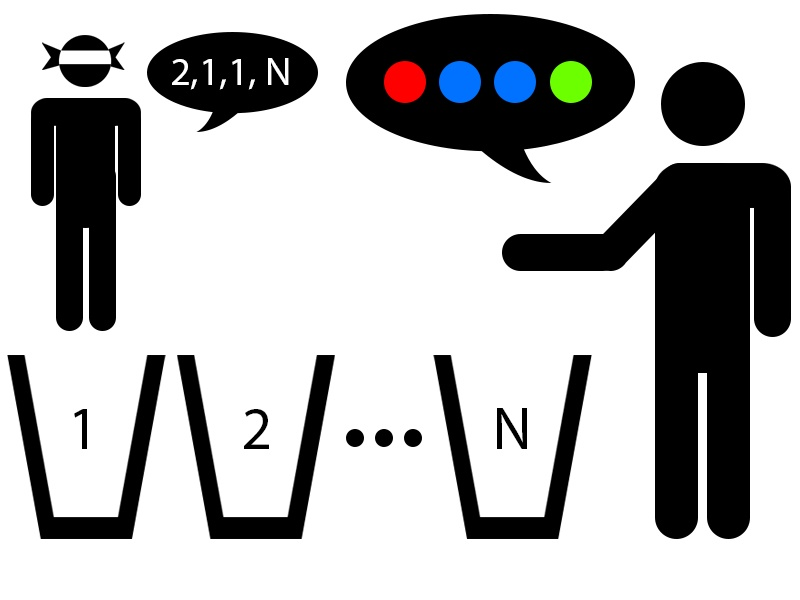
\includegraphics[scale=0.7]{img/hmm.jpg}
\caption{Иллюстрация процесса, описываемого СММ}
\end{figure}
Используя СММ для описания этого процесса первый человек может пытаться угадывать из какой урны, какой шар был взят. Наблюдаемым процессом в данном случае является речь человека, называющего цвета взятых шаров, а скрытым процессом являетсе его выбор той или иной урны. В этой ситуации элементами множества наблюдений являются цвета шаров, а элементами множества скрытых состояний являются номера урн.

\subsubsection{Использование скрытой марковской модели для разметки текста}
Текст на естественном языке так же можно рассматривать как два стохастических процесса, описываемых скрытой марковской моделью. В таком случае наблюдаемым процессом можно считать последовательность символов текста, а скрытым процессом - принадлежность того или иного символа словоформе, ее границе или непринадлежность символа словоформе. Возможно введение дополнительных скрытых состояний для описания различных типов словоформ. Множество наблюдений представляет собой типы символов, из которых состоит текст. В простейшем случае множество наблюдений может представлять собой подмножество кодов символов некоторой кодировочной таблицы. 

\subsubsection{Обучение скрытой марковской модели с учителем}
Как было упомянуто выше, алгоритм Баума-Велша является обучением 

\subsubsection{Корпусная лингвистика}

\subsection{Фаза словарного поиска}